\chapter{Results}
\label{Results}
\section{Experiment Description}
To demonstrate our results, we plotted results from one standardized run of multiple division configurations trained over 2'000 rounds of 10'000 hands each, for a total of 20'000'000 hands.

All divisions included one random and one call agent as baselines, and all divisions cloned a new generation of teachers every 200 rounds, for a total of 90 agents over the whole run. Table \ref{RunDivisions} shows the different training division configurations.

\begin{table}[h!]
\centering
\begin{tabular}{|| c | c | c ||} 
 \hline
 Name & Matchup Method & Agents \\ [0.5ex] 
 \hline\hline
 Qln8-Cl & Climbing & Qlearn-8 \\
 QlnA-Cl & Climbing & Qlearn-All \\
 SacL-Cl & Climbing & Sac-Low \\
 SacH-Cl & Climbing & Sac-High \\
 AllAg-Cl & Climbing & Qlearn-8, Qlearn-All, Sac-Low, Sac-High \\
 QlnA-Rn & Random & Qlearn-All \\ [1ex] 
 \hline
\end{tabular}
\caption{Training division configurations used in the standardized run}
\label{RunDivisions}
\end{table}

We trained on a computer with an Intel 6770k CPU, 16GB Ram, and an Nvidia 1070GTX GPU with 8GB VRAM. The training process took about 44 hours in real-time.

After training, we ran three PermaEval divisions to evaluate all agents according to the various metrics: one for all the winnings-based metrics, one for across-division TrueSkill, and a second TrueSkill to evaluate its consistency.

We computed winnings with 10'000 hands per agent pairing of all 102 agents, for a total of 52'020'000 hands. For fairness of comparison, TrueSkill was evaluated for 5'300 rounds, which is approximately the same number of hands.


\section{Performance Metrics}

First, we compare different metrics in consistency and strategy clustering, and take a closer look at TrueSkill.

\subsection{Leaderboards}

\begin{table}[H]
\centering
\subcaptionbox{Sorted by TrueSkill (TS)}{
\begin{tabular}{|| c | c | c | c | c ||} 
 \hline
 Name & TS & Mean & Med & 20-Pctl \\ [0.5ex] 
 \hline\hline
     exam &     151.04 &  3.26 &    2.35 &           0.21 \\
    radar &     148.97 &  2.79 &    2.02 &           0.14 \\
     loss &     146.49 &  3.95 &    2.76 &           0.33 \\
      tan &     143.41 &  4.47 &    2.55 &           0.19 \\
    brick &     142.55 &  5.13 &    2.65 &           0.35 \\
     clam &     142.43 &  4.67 &    2.81 &           0.15 \\
   seeker &     141.14 &  6.16 &    2.98 &           0.33 \\
   wisdom &     140.39 &  1.47 &    0.94 &           0.06 \\
 suitcase &     138.85 &  4.81 &    2.45 &           0.33 \\
   flight &     138.73 &  4.58 &    2.53 &           0.23 \\ [1ex] 
 \hline
\end{tabular}
}
\subcaptionbox{Sorted by Mean
}{
\begin{tabular}{|| c | c | c | c | c ||} 
 \hline
 Name & TS & Mean & Med & 20-Pctl \\ [0.5ex] 
 \hline\hline
   orange &     129.16 &  6.79 &    1.32 &          -0.07 \\
     watt &     133.09 &  6.59 &    2.24 &           0.23 \\
   seeker &     141.14 &  6.16 &    2.98 &           0.33 \\
 ecclesia &     124.79 &  6.15 &    1.42 &           0.00 \\
   config &     122.43 &  6.06 &    0.89 &          -1.20 \\
    power &     132.34 &  6.04 &    1.58 &           0.00 \\
  creator &     134.82 &  5.91 &    2.59 &           0.03 \\
    union &     129.96 &  5.65 &    1.50 &           0.01 \\
  cowbell &     118.01 &  5.50 &    0.88 &          -2.32 \\
     yarn &     119.79 &  5.50 &    1.14 &          -1.60 \\ [1ex] 
 \hline
\end{tabular}
}
\subcaptionbox{Sorted by Median (Med)
}{
\begin{tabular}{|| c | c | c | c | c ||} 
 \hline
 Name & TS & Mean & Med & 20-Pctl \\ [0.5ex] 
 \hline\hline
   seeker &     141.14 &  6.16 &    2.98 &           0.33 \\
     clam &     142.43 &  4.67 &    2.81 &           0.15 \\
  penguin &     135.08 &  5.22 &    2.76 &           0.00 \\
     loss &     146.49 &  3.95 &    2.76 &           0.33 \\
    brick &     142.55 &  5.13 &    2.65 &           0.35 \\
  creator &     134.82 &  5.91 &    2.59 &           0.03 \\
      tan &     143.41 &  4.47 &    2.55 &           0.19 \\
   flight &     138.73 &  4.58 &    2.53 &           0.23 \\
 suitcase &     138.85 &  4.81 &    2.45 &           0.33 \\
     exam &     151.04 &  3.26 &    2.35 &           0.21 \\[1ex] 
 \hline
\end{tabular}
}
\subcaptionbox{Sorted by 20-Percentile (20-Pctl)
}{
\begin{tabular}{|| c | c | c | c | c ||} 
 \hline
 Name & TS & Mean & Med & 20-Pctl \\ [0.5ex] 
 \hline\hline
    brick &     142.55 &  5.13 &    2.65 &           0.35 \\
 suitcase &     138.85 &  4.81 &    2.45 &           0.33 \\
     loss &     146.49 &  3.95 &    2.76 &           0.33 \\
   seeker &     141.14 &  6.16 &    2.98 &           0.33 \\
     watt &     133.09 &  6.59 &    2.24 &           0.23 \\
   flight &     138.73 &  4.58 &    2.53 &           0.23 \\
     exam &     151.04 &  3.26 &    2.35 &           0.21 \\
      tan &     143.41 &  4.47 &    2.55 &           0.19 \\
     rain &     135.02 &  4.20 &    1.01 &           0.17 \\
     clam &     142.43 &  4.67 &    2.81 &           0.15 \\[1ex] 
 \hline
\end{tabular}
}
\caption{Top 10 agents on leaderboard sorted by each metric}
\label{TableTopAgentsMetrics}
\end{table}

We can see in Table \ref{TableTopAgentsMetrics} that the four metrics we used disagree on which agents were best. There are a handful of agents (e.g. \textit{seeker}, \textit{exam}, \textit{brick}, or \textit{suitcase}) that show up in most leaderboards near the top, and it is from these agents that we selected candidates for the AIcrowd competition (specifically, \textit{seeker} was our final agent), but overall there is substantial disagreement.

As one might expect, mean diverges from the other metrics most. We believe this is because mean does not reward consistency, e.g. losing a bit often and winning big sometimes is a good strategy for mean optimization. All three other metrics discourage it, and reward worst-case consistency.
\begin{figure}[H]
\centering
\subcaptionbox{
    Colored by TrueSkill
}{
    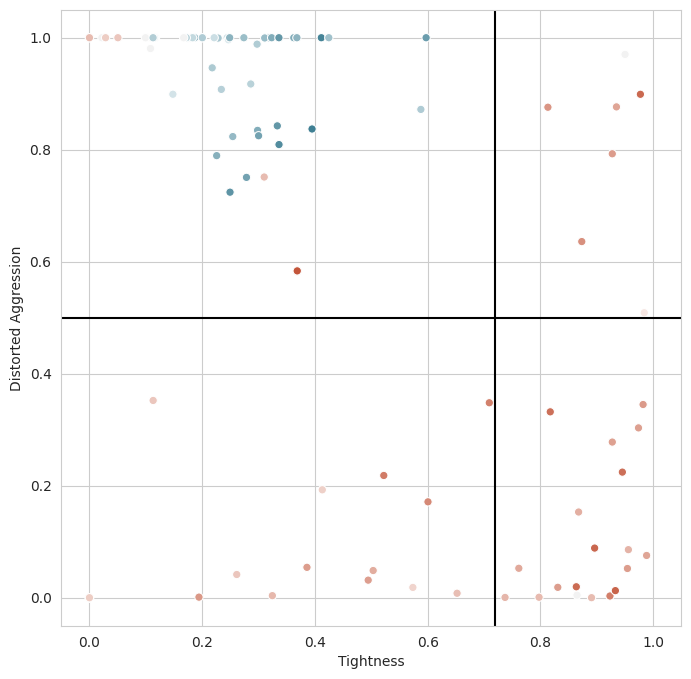
\includegraphics[width=0.45\linewidth]{Results/figures/aggtightrankTrueSkill.png}
}
\subcaptionbox{
    Colored by Mean
}{
    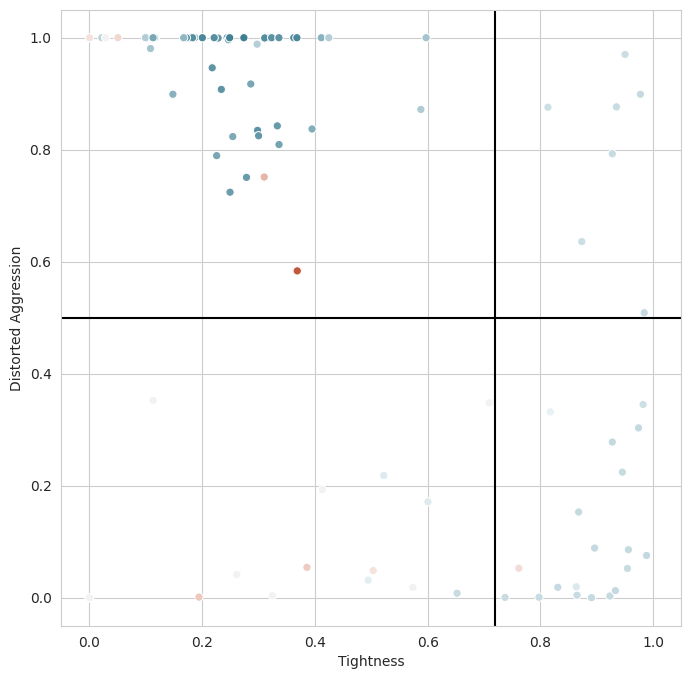
\includegraphics[width=0.45\linewidth]{Results/figures/aggtightrankMean.png}
}
\subcaptionbox{
    Colored by Median
}{
    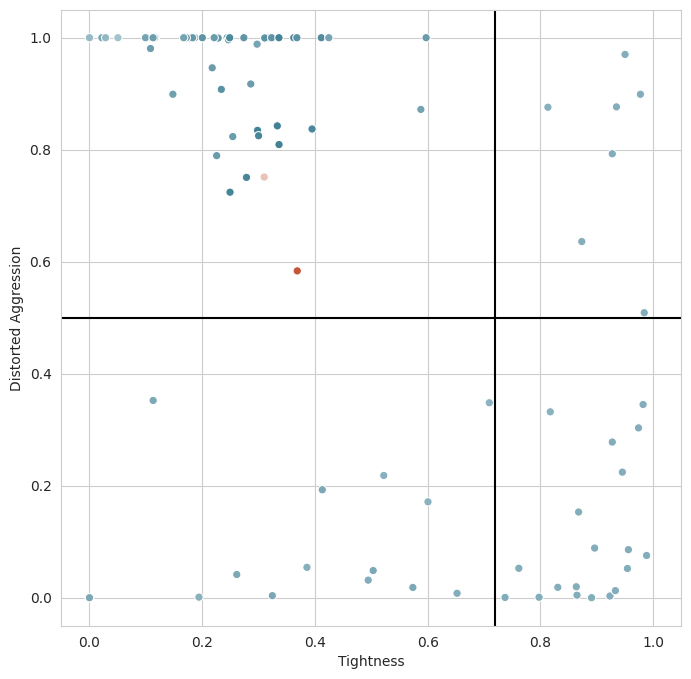
\includegraphics[width=0.45\linewidth]{Results/figures/aggtightrankMedian.png}
}
\subcaptionbox{
    Colored by 20-Percentile
}{
    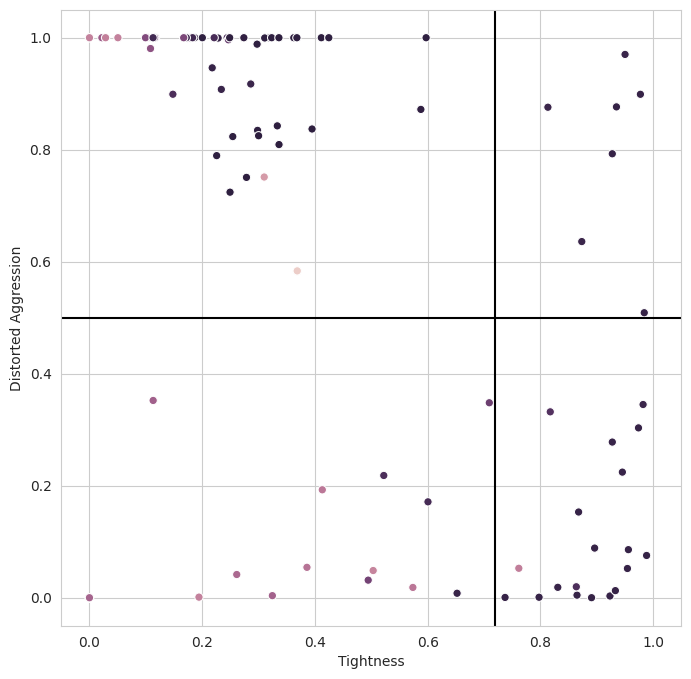
\includegraphics[width=0.45\linewidth]{Results/figures/aggtightrank20-Percentile.png}
}
\caption{Aggression and Tightness colored by rank for each metric, blue is better (normalized)}
\label{AggTightRank}
\end{figure}

However, this difference is not visible in the strategy plots seen in Figure \ref{AggTightRank}. Instead here it is TrueSkill that is an outlier, as it ranks tight and passive agents as worse overall than all others, though mean also considers them worse than the other two.

This would lead to the hypothesis that tight and passive players, which we will see later (section \ref{ResultsAgents}) are mostly SAC agents, play consistently ok in their worst games (decent 20pctl and median), but rarely take advantage of good games (low mean), and also rarely win matches (low TrueSkill). This is consistent with the definition of passivity and tightness, though one would expect the aggressive and loose players to have lower 20pctl scores, which we do not observe.


\begin{figure}[H]
\centering
    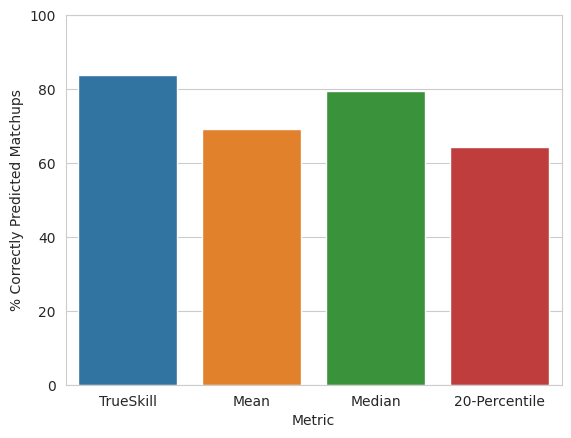
\includegraphics[width=0.8\linewidth]{Results/figures/upsets_per_metric.png}
\caption{Percent 1v1 evaluations whose outcome matches what the metric difference predicts}
\label{UpsetsPlot}
\end{figure}

Figure \ref{UpsetsPlot} demonstrates how good these metrics are at predicting the winner in a 3v3 evaluation. We can see that TrueSkill as the only metric specifically optimizing for win probability performs best, closely followed by median.


\subsection{TrueSkill Coherence}

\begin{figure}[H]
\centering
\subcaptionbox{
    First PermaEval division TrueSkill
}{
    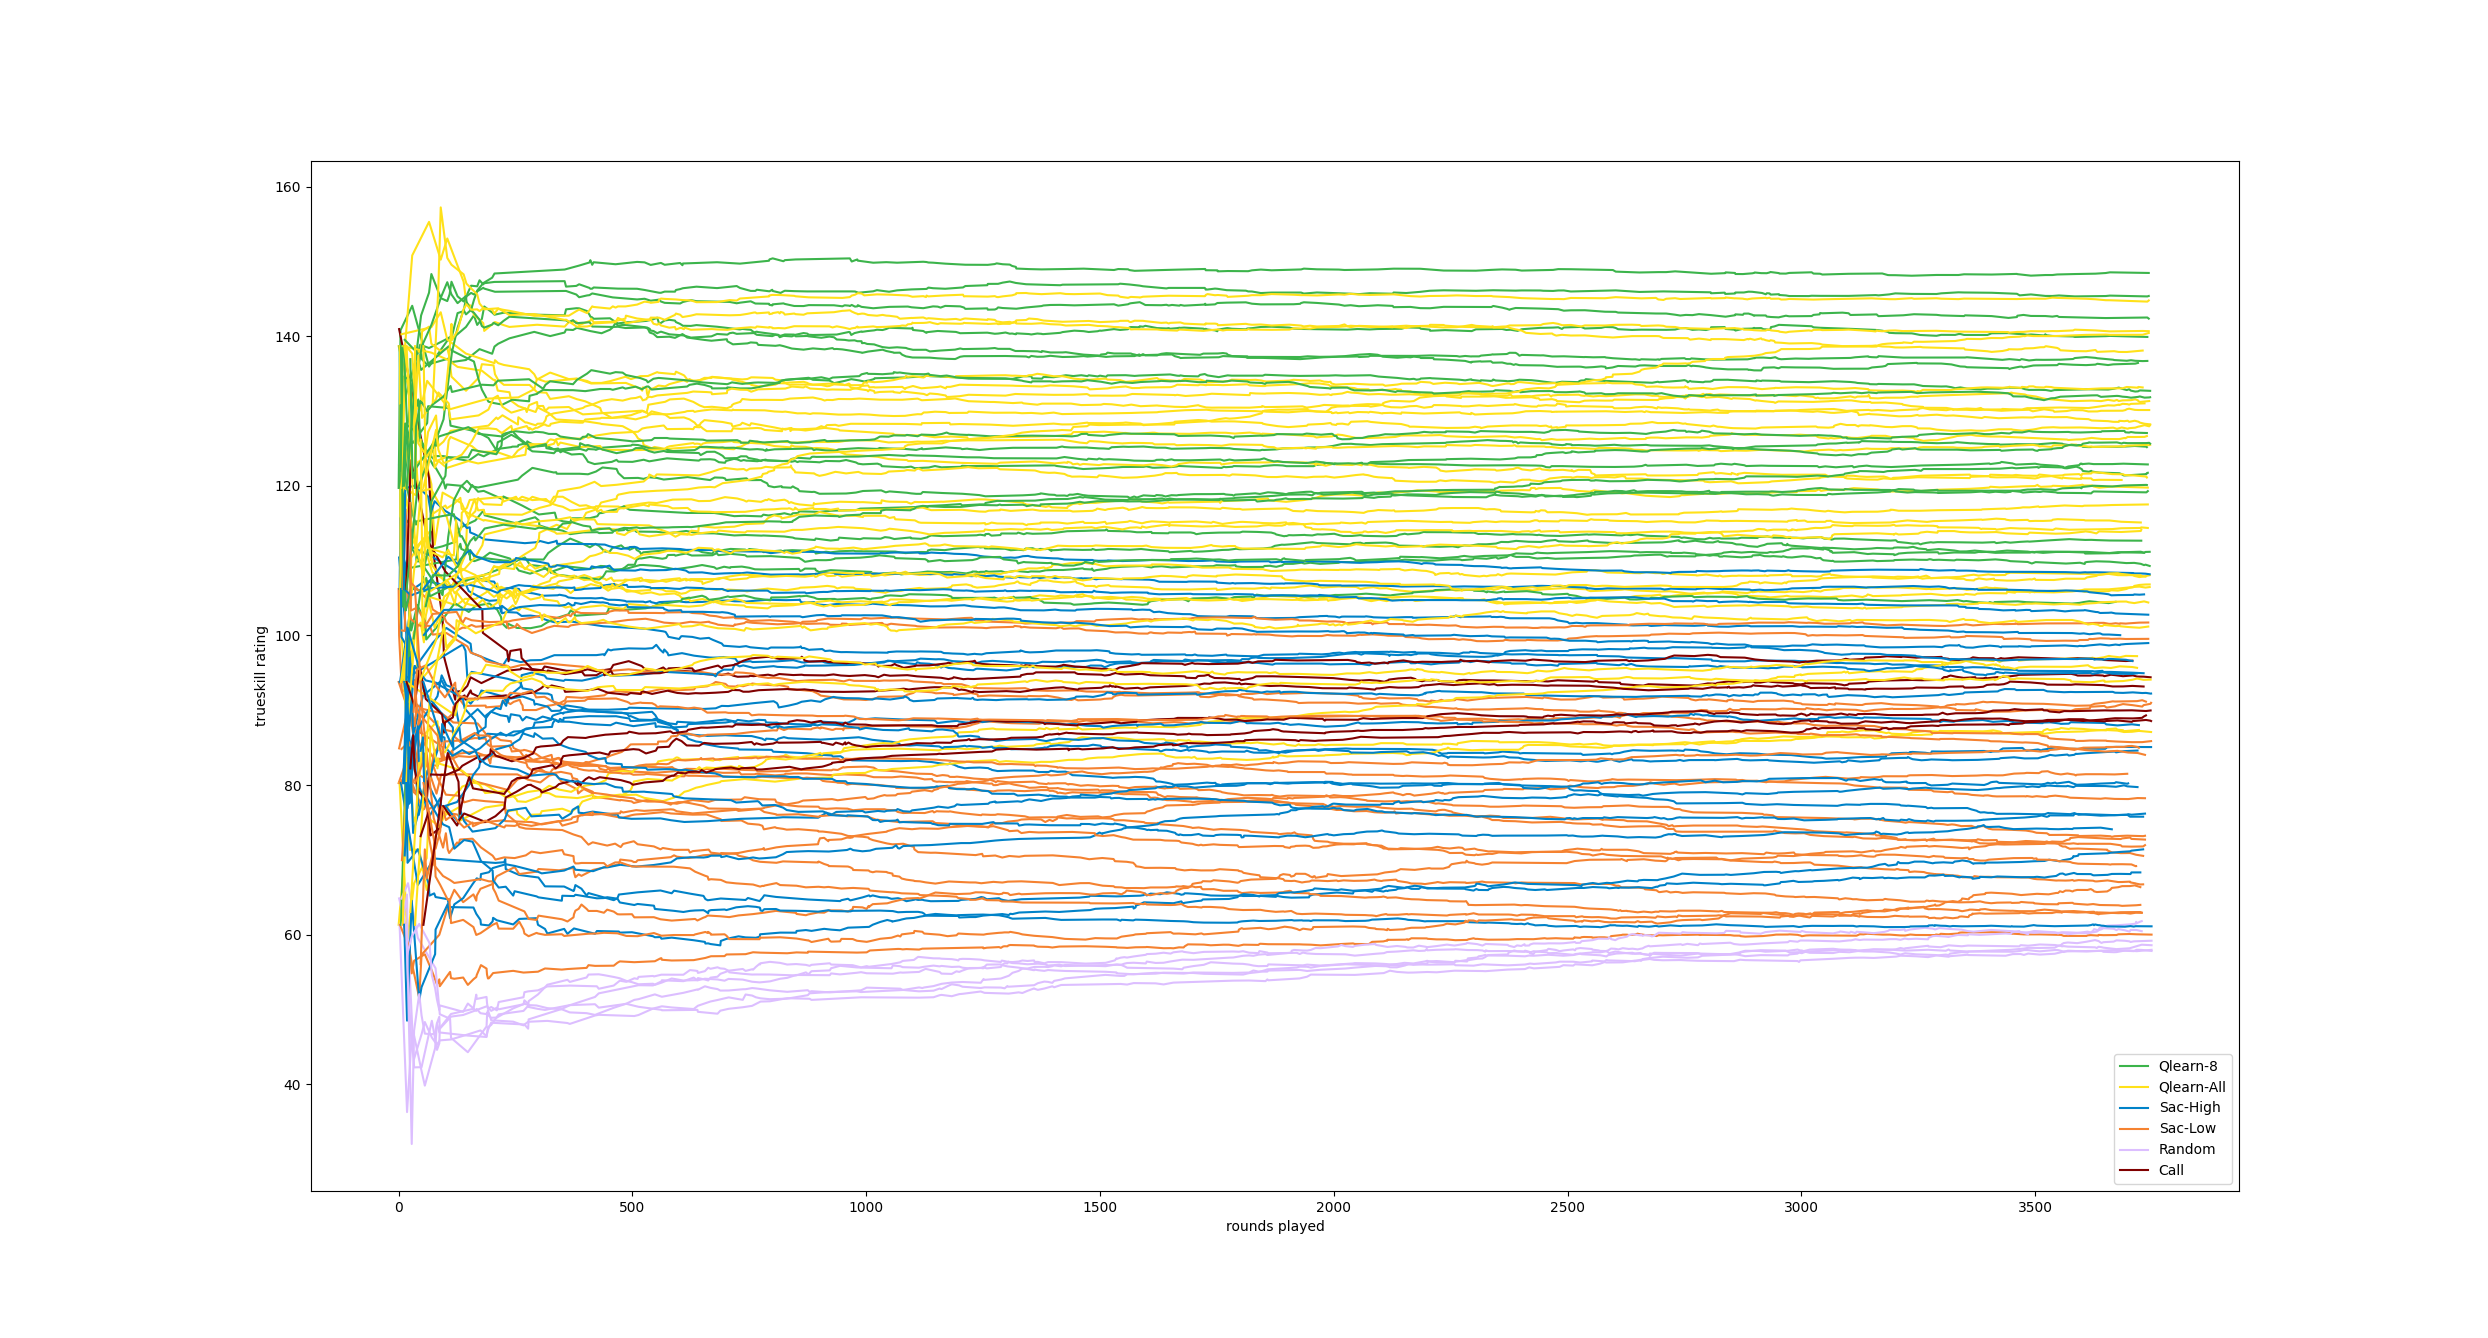
\includegraphics[width=0.85\linewidth]{Results/figures/trueskill1.png}
}
\subcaptionbox{
    Second PermaEval division TrueSkill
}{
    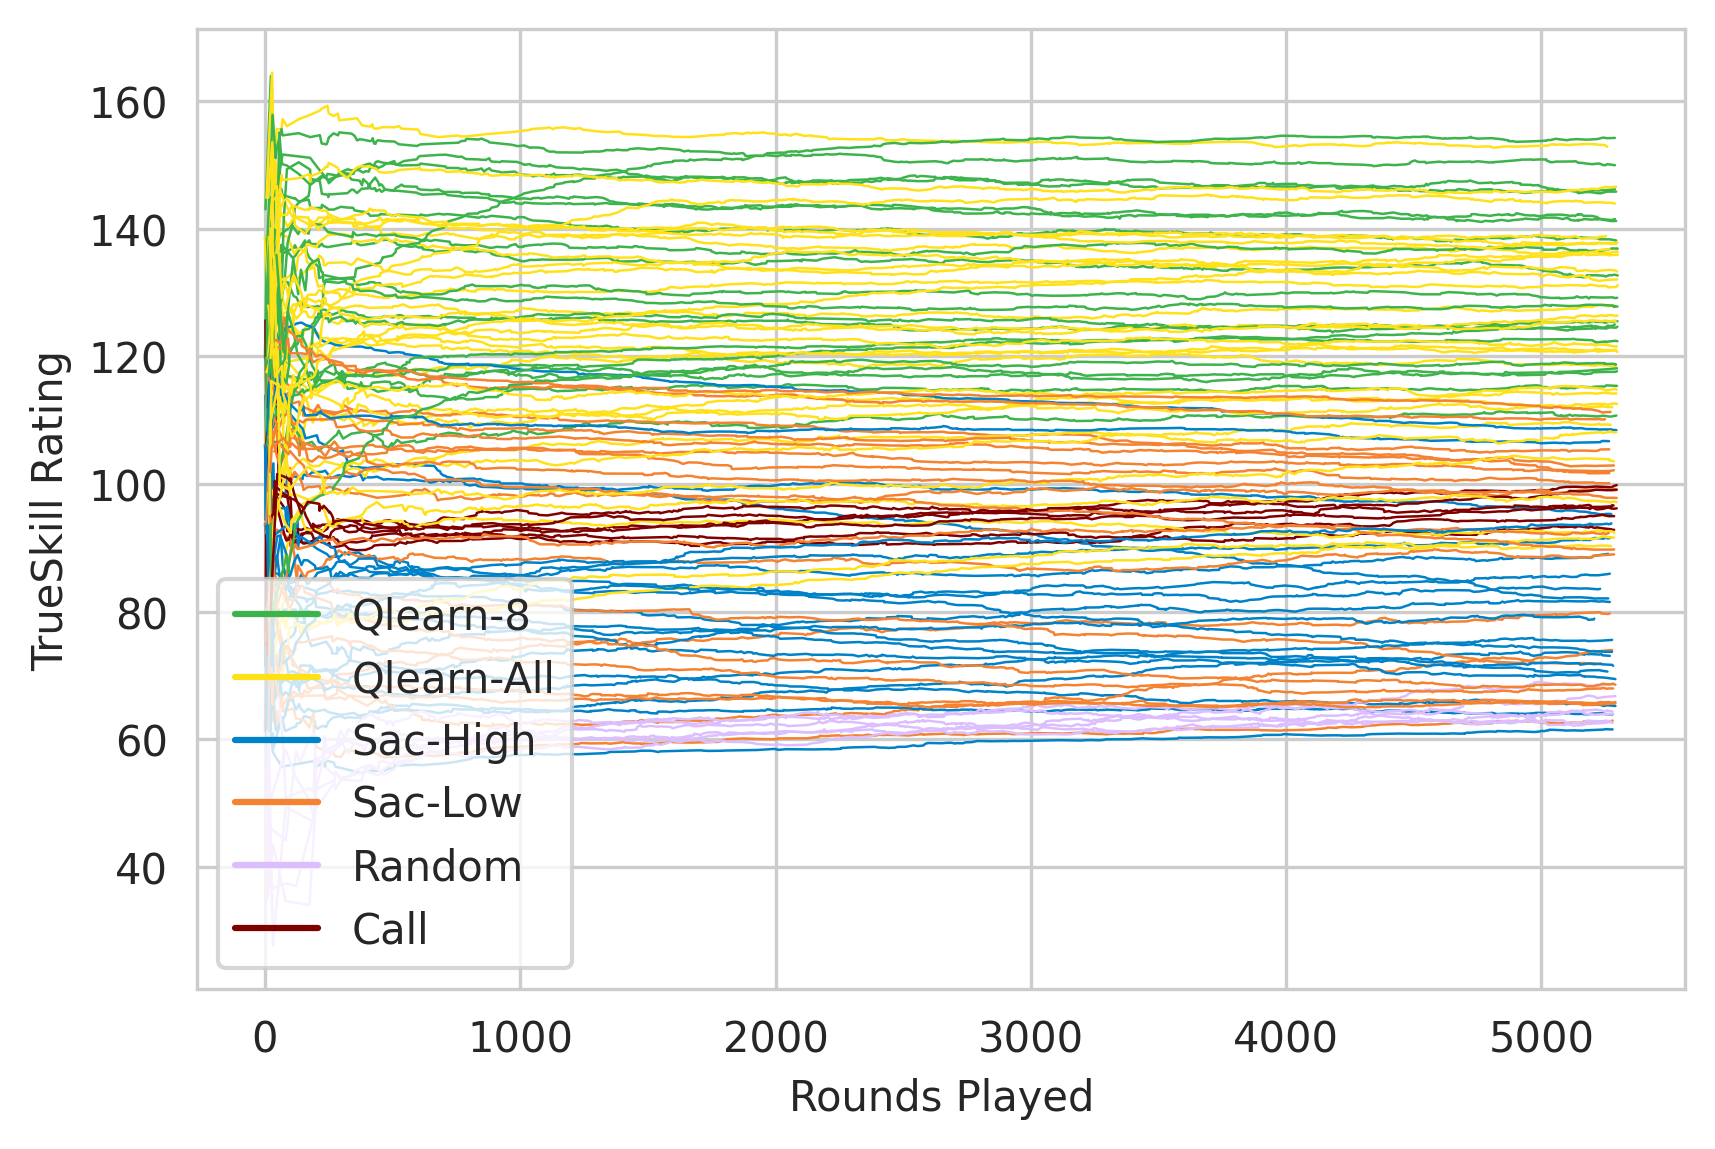
\includegraphics[width=0.85\linewidth]{Results/figures/trueskill2.png}
}
\caption{TrueSkill over time in both PermaEval divisions}
\label{TrueSkillCompare}
\end{figure}

TrueSkill did not converge quickly or well in preliminary experiments, so to establish that it is at least consistent we computed the full ranking twice. Both runs with the changing TrueSkill estimates can be seen in Figure \ref{TrueSkillCompare}.

While the broad tendencies stabilize quickly, we still observe agents swapping or even completely changing their skill rating by as much as 40 points after the first 500 rounds, despite all agents being static and always playing at the same skill level. This does not bode well for convergence.

\begin{figure}[H]
\centering
    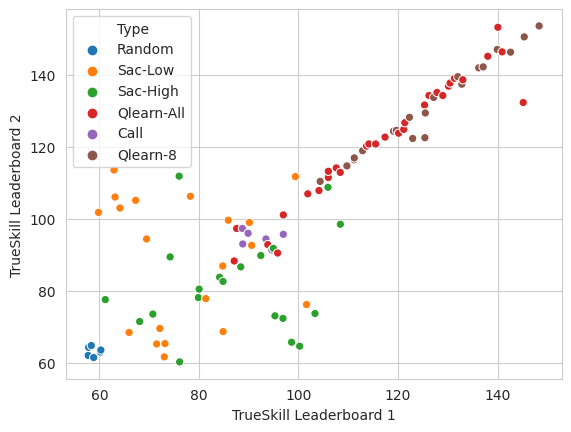
\includegraphics[width=0.8\linewidth]{Results/figures/trueskill_comparison.png}
\caption{Agent rank in both TrueSkill PermaEval divisions, colored by type}
\label{TrueSkillCompare2}
\end{figure}

Figure \ref{TrueSkillCompare2} shows the rank of all agents as estimated by the two runs of TrueSkills. Were TrueSkill perfectly consistent, this would be a straight line. Instead we see a mystifying result of it being dependent on agent types; SAC agents appear to play inconsistently when judged by TrueSkill (i.e. ranking after matches), but other agents are consistent, if not perfectly so. This seems less an artifact of TrueSkill and more an issue with SAC agents themselves.

\section{Agents}
\label{ResultsAgents}
How do the different agent architectures compare?

\begin{figure}[H]
\centering
    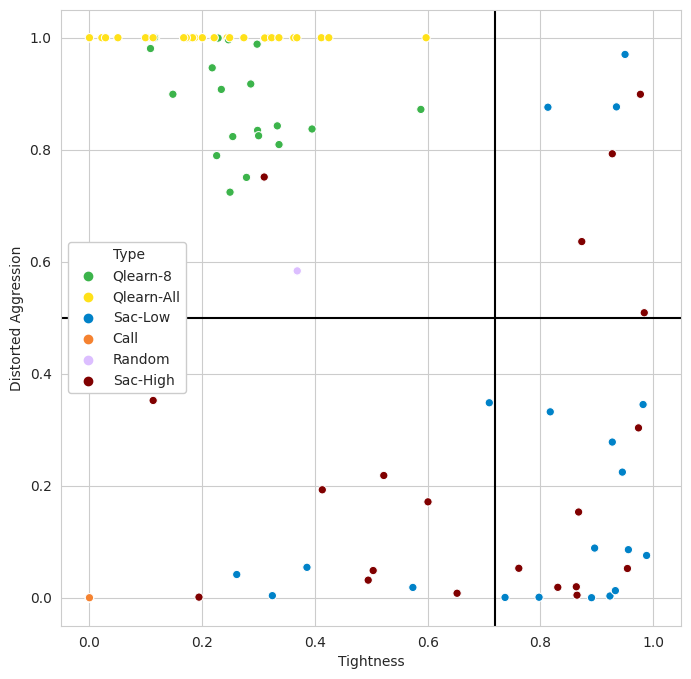
\includegraphics[width=0.8\linewidth]{Results/figures/traditional_scatterplot_Type.png}
\caption{Aggression and Tightness, colored by agent type}
\label{AggTightAgentType}
\end{figure}

Agent architectures appear paramount for their strategy. Figure \ref{AggTightAgentType} shows results from multiple divisions (i.e. different seeds and different opponents), which does not prevent a remarkable convergence by agent type.

We see that Qlearn-All almost never calls, and either folds or raises, leaning towards more raises. Qlearn-8 shares a similar tendency but not nearly as strong (the scale of \textit{Distorted Aggression} is hyperbolic towards the top). We believe this is because of implementation details of exploration, more in section \ref{ConclusionAgents}.

In contrast, SAC agents play aggressive only when tight, or loose when passive. This is more "sensible" by common sense (if you call less, you fold more), but appears to perform worse in our leagues.

\begin{table}[H]
\centering
\begin{tabular}{|| c | c | c | c | c ||} 
 \hline
 Rank & TrueSkill & Mean & Median & 20-Percentile \\ [0.5ex] 
 \hline\hline
   1 &    Qlearn-8 &  Qlearn-All &  Qlearn-All &    Qlearn-All \\
   2 &  Qlearn-All &  Qlearn-All &    Qlearn-8 &    Qlearn-All \\
   3 &    Qlearn-8 &  Qlearn-All &    Qlearn-8 &      Qlearn-8 \\
   4 &    Qlearn-8 &  Qlearn-All &    Qlearn-8 &      Qlearn-8 \\
   5 &  Qlearn-All &  Qlearn-All &  Qlearn-All &    Qlearn-All \\
   6 &    Qlearn-8 &  Qlearn-All &  Qlearn-All &      Qlearn-8 \\
   7 &  Qlearn-All &  Qlearn-All &    Qlearn-8 &      Qlearn-8 \\
   8 &  Qlearn-All &  Qlearn-All &    Qlearn-8 &      Qlearn-8 \\
   9 &    Qlearn-8 &  Qlearn-All &    Qlearn-8 &    Qlearn-All \\
  10 &    Qlearn-8 &  Qlearn-All &    Qlearn-8 &      Qlearn-8 \\
  11 &    Qlearn-8 &  Qlearn-All &  Qlearn-All &    Qlearn-All \\
  12 &  Qlearn-All &  Qlearn-All &  Qlearn-All &    Qlearn-All \\
  13 &  Qlearn-All &    Qlearn-8 &  Qlearn-All &      Qlearn-8 \\
  14 &  Qlearn-All &  Qlearn-All &    Qlearn-8 &    Qlearn-All \\
  15 &    Qlearn-8 &    Qlearn-8 &  Qlearn-All &    Qlearn-All \\
  16 &  Qlearn-All &    Qlearn-8 &    Qlearn-8 &      Qlearn-8 \\
  17 &  Qlearn-All &    Qlearn-8 &  Qlearn-All &    Qlearn-All \\
  18 &    Qlearn-8 &    Qlearn-8 &  Qlearn-All &    Qlearn-All \\
  19 &  Qlearn-All &    Qlearn-8 &  Qlearn-All &    Qlearn-All \\
  20 &  Qlearn-All &    Qlearn-8 &  Qlearn-All &    Qlearn-All \\[1ex] 
 \hline
\end{tabular}
\caption{Agent type of the top 20 agents according to each metric}
\label{TypeRankings}
\end{table}

Looking at Table \ref{TypeRankings} the first immediate observation is that no architecture other than the two Qlearns was able to compete.

The second is that while Qlearn-8 and Qlearn-All seem approximately evenly matched in most metrics, in mean Qlearn-All is dominant, earning more money on average despite not winning more often. This is consistent with Qlearn-All's higher aggression.

\begin{figure}[H]
\centering
\subcaptionbox{
    Ranked by TrueSkill
}{
    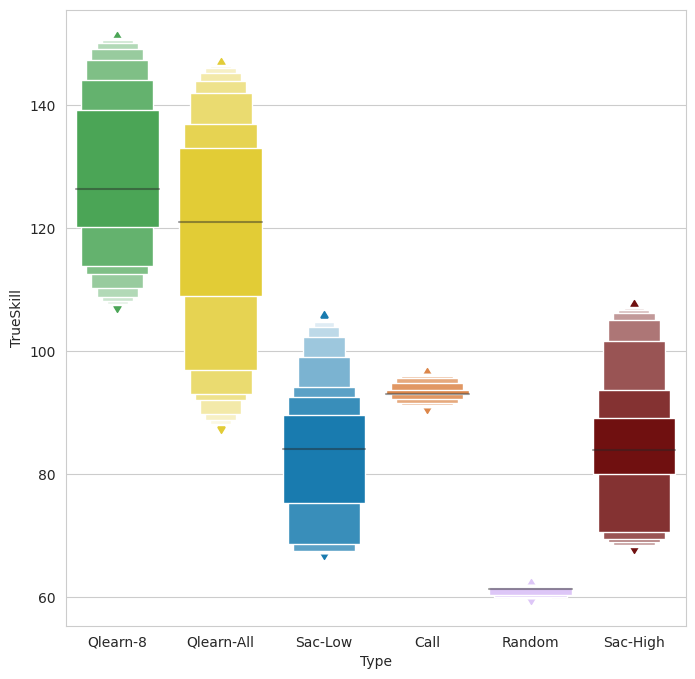
\includegraphics[width=0.45\linewidth]{Results/figures/agentdistTrueSkill.png}
}
\subcaptionbox{
    Ranked by Mean
}{
    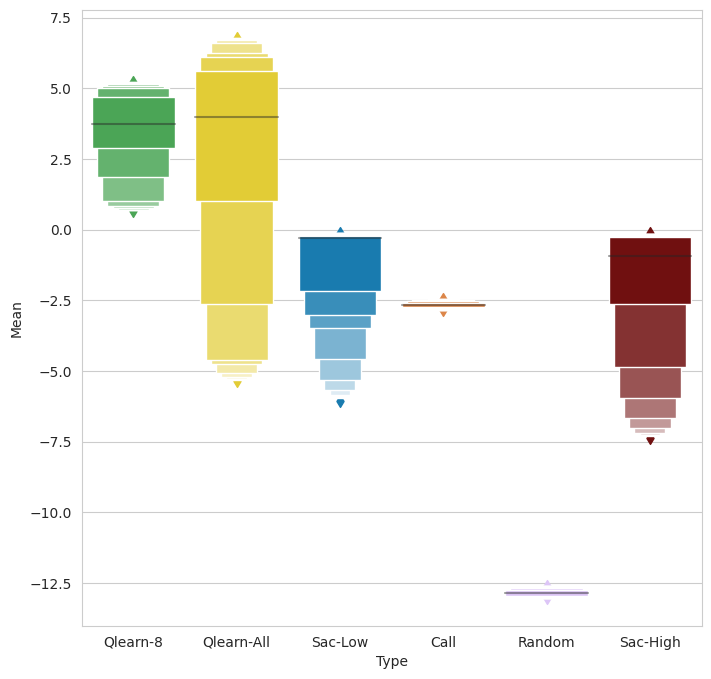
\includegraphics[width=0.45\linewidth]{Results/figures/agentdistMean.png}
}
\subcaptionbox{
    Ranked by Median
}{
    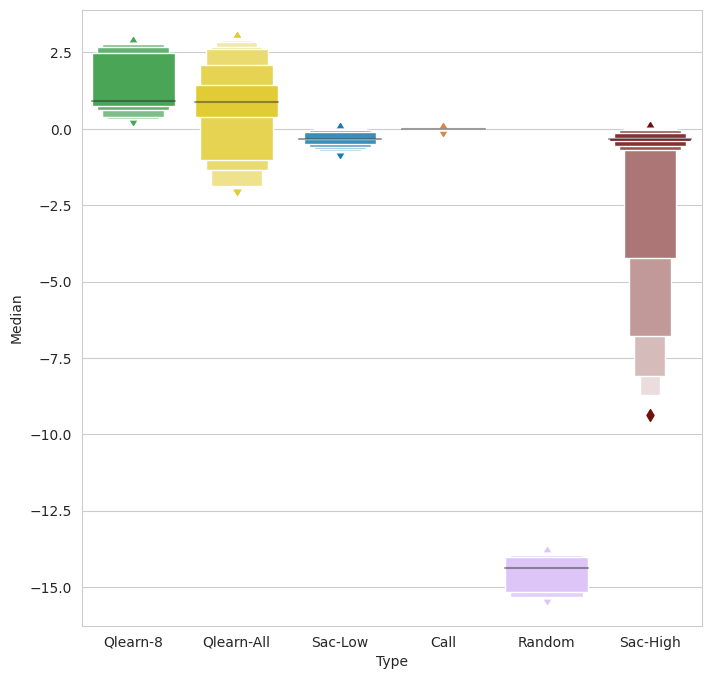
\includegraphics[width=0.45\linewidth]{Results/figures/agentdistMedian.png}
}
\subcaptionbox{
    Ranked by 20-Percentile
}{
    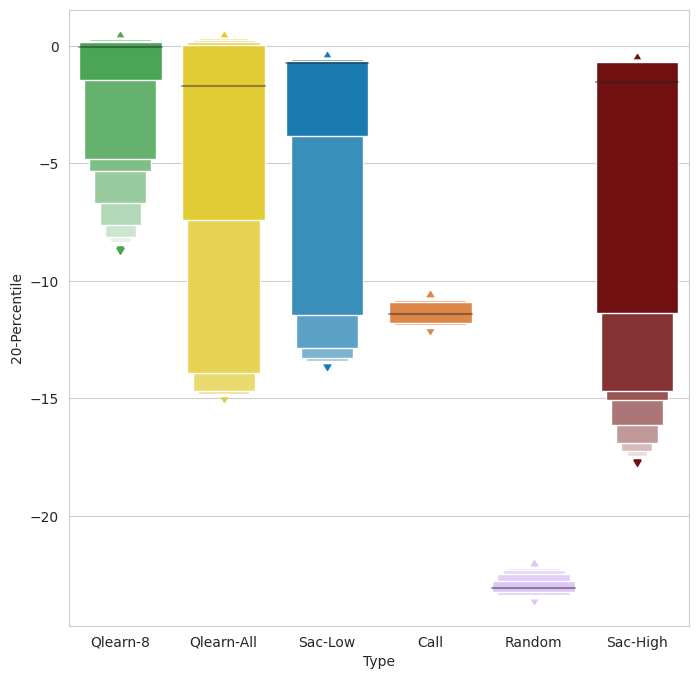
\includegraphics[width=0.45\linewidth]{Results/figures/agentdist20-Percentile.png}
}
\caption{Agent distribution by type and rank}
\label{AgentTypeDistribution}
\end{figure}

Figure \ref{AgentTypeDistribution} shows how the relative performance of SAC agents differs depending on metrics; ranked by mean or median they outperform call agents, but ranked by TrueSkill only the best of them do.

We can also see that 20pctl is left-skewed, with the best agents being closer to the norm than the worst agents. This makes it difficult to compare the best half, but it allows some insight in the worst; we see that Qlearn-All is surprisingly good, even with its worst untrained agents, in its worst 20\% of matches, despite extreme aggression.

\begin{figure}[H]
\centering
\subcaptionbox{
    Ranked by TrueSkill
}{
    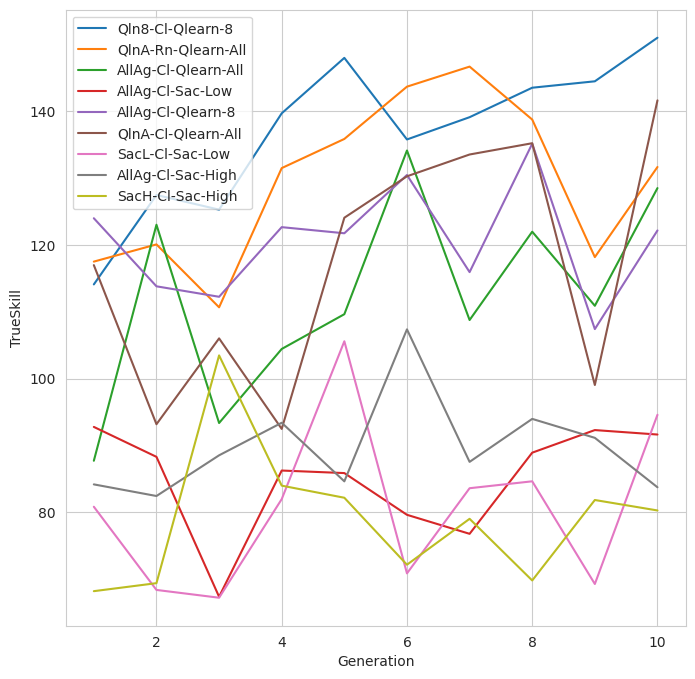
\includegraphics[width=0.45\linewidth]{Results/figures/generationsTrueSkill.png}
}
\subcaptionbox{
    Ranked by Mean
}{
    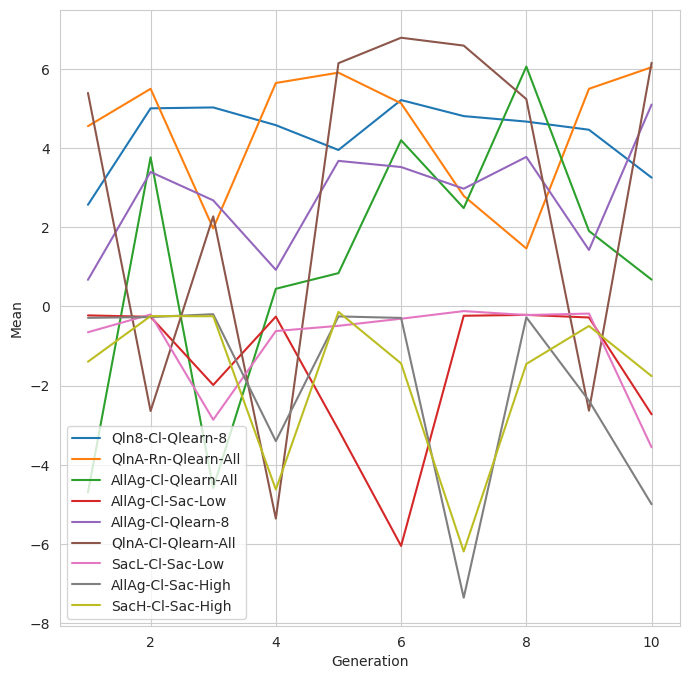
\includegraphics[width=0.45\linewidth]{Results/figures/generationsMean.png}
}
\subcaptionbox{
    Ranked by Median
}{
    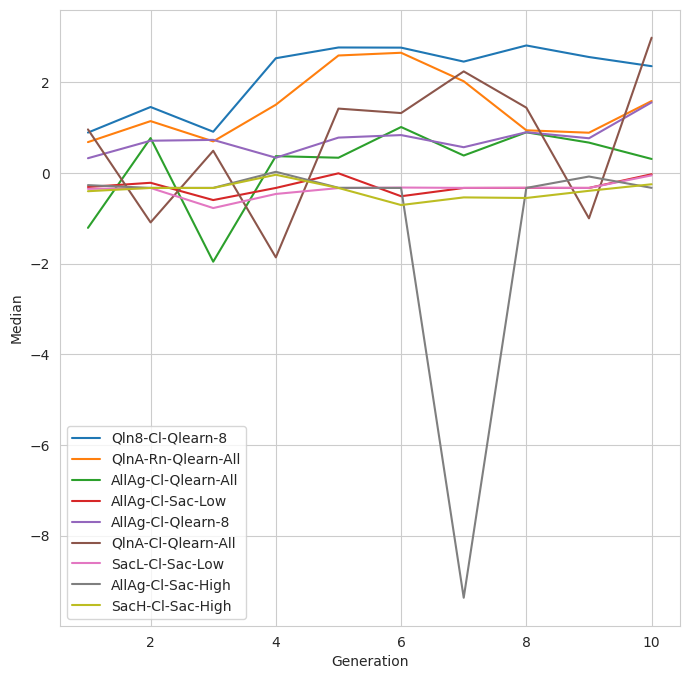
\includegraphics[width=0.45\linewidth]{Results/figures/generationsMedian.png}
}
\subcaptionbox{
    Ranked by 20-Percentile
}{
    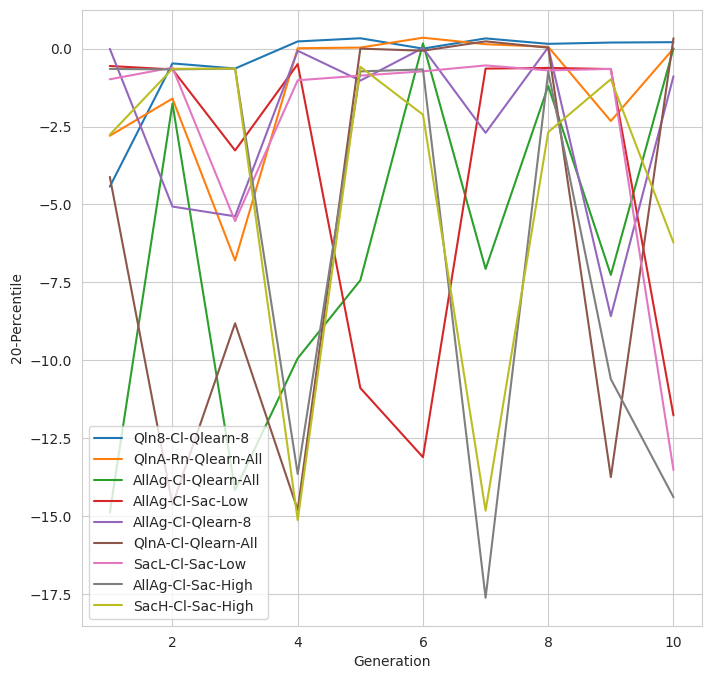
\includegraphics[width=0.45\linewidth]{Results/figures/generations20-Percentile.png}
}
\caption{Agent evolution over time by type and rank}
\label{AgentGenerations}
\end{figure}

Each agent left clones of itself every 200 iterations. Comparing these clones by generation allows us to see how agents improved over time. Figure \ref{AgentGenerations} shows this progress using the four metrics.

On first sight, it looks like they haven't. Improvement is visible in TrueSkill for the Qlearn agents, as well as small improvements in the other metrics, but overall this is less improvement than expected.



\section{Populations}

How important are division populations?

\begin{table}[H]
\centering
\begin{tabular}{|| c | c | c | c | c ||} 
 \hline
 Rank & TrueSkill & Mean & Median & 20-Percentile \\ [0.5ex] 
 \hline\hline
   1 &   Qln8-Cl &   QlnA-Cl &   QlnA-Cl &       QlnA-Rn \\
   2 &   QlnA-Rn &   QlnA-Cl &   Qln8-Cl &       QlnA-Cl \\
   3 &   Qln8-Cl &   QlnA-Cl &   Qln8-Cl &       Qln8-Cl \\
   4 &   Qln8-Cl &   QlnA-Cl &   Qln8-Cl &       Qln8-Cl \\
   5 &   QlnA-Rn &  AllAg-Cl &   QlnA-Rn &       QlnA-Cl \\
   6 &   Qln8-Cl &   QlnA-Rn &   QlnA-Rn &       Qln8-Cl \\
   7 &   QlnA-Cl &   QlnA-Rn &   Qln8-Cl &       Qln8-Cl \\
   8 &   QlnA-Rn &   QlnA-Rn &   Qln8-Cl &       Qln8-Cl \\
   9 &   Qln8-Cl &   QlnA-Rn &   Qln8-Cl &      AllAg-Cl \\
  10 &   Qln8-Cl &   QlnA-Rn &   Qln8-Cl &       Qln8-Cl \\
  11 &   Qln8-Cl &   QlnA-Cl &   QlnA-Cl &       QlnA-Rn \\
  12 &   QlnA-Cl &   QlnA-Cl &   QlnA-Rn &       QlnA-Rn \\
  13 &  AllAg-Cl &   Qln8-Cl &   QlnA-Rn &      AllAg-Cl \\
  14 &   QlnA-Rn &   QlnA-Rn &  AllAg-Cl &       QlnA-Rn \\
  15 &  AllAg-Cl &  AllAg-Cl &   QlnA-Rn &       QlnA-Cl \\
  16 &   QlnA-Cl &   Qln8-Cl &   Qln8-Cl &      AllAg-Cl \\
  17 &   QlnA-Rn &   Qln8-Cl &   QlnA-Cl &       QlnA-Rn \\
  18 &  AllAg-Cl &   Qln8-Cl &   QlnA-Cl &      AllAg-Cl \\
  19 &   QlnA-Rn &   Qln8-Cl &   QlnA-Cl &       QlnA-Cl \\
  20 &   QlnA-Cl &   Qln8-Cl &   QlnA-Rn &       QlnA-Rn \\ [1ex] 
 \hline
\end{tabular}
\caption{Agent division of the top 20 agents according to each metric}
\label{DivisionRankings}
\end{table}

According to Table \ref{DivisionRankings} Climbing appears only marginally better than Random matching, though enough to be relevant. This accords with smaller experiments we did before this run. It also seems that mixing all agents decreases performance overall, indicating that overfitting is not (yet) an issue. It might be that competition against better agents is important, but its relative under-performance may also be a symptom of its lower training time; because the mixed division has more agents, the training rounds are split between them, leaving each individual agent with less rounds per cloning generation.

\begin{figure}[H]
\centering
    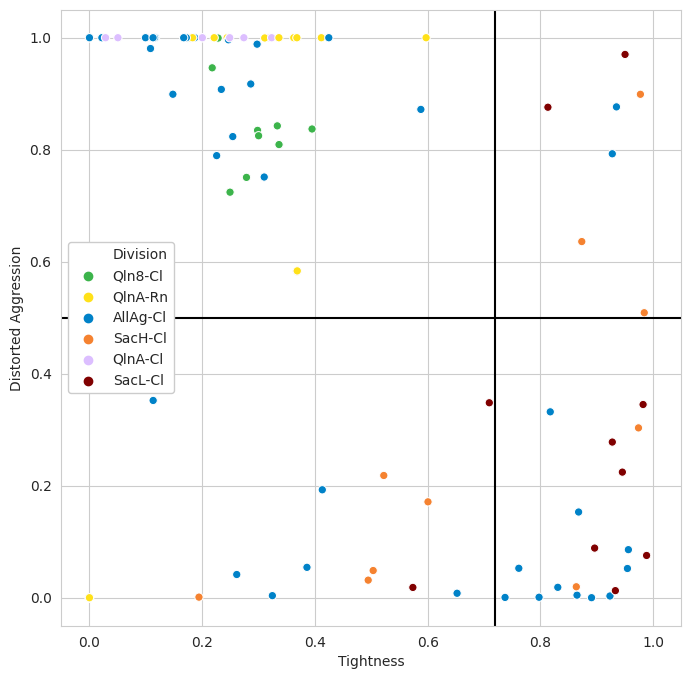
\includegraphics[width=0.8\linewidth]{Results/figures/traditional_scatterplot_Division.png}
\caption{Aggression and Tightness, colored by division}
\label{AggTightDivision}
\end{figure}

Compared with Figure \ref{AggTightAgentType}, Figure \ref{AggTightDivision} is more mixed. In particular, the mixed division (AllAg-Cl) is spread across the entire plot, and each division specialized to an architecture covers the area of that architecture. This reinforces the concept that strategy space location depends mostly on architecture choice and not on population.

\begin{figure}[H]
\centering
\subcaptionbox{
    Ranked by TrueSkill
}{
    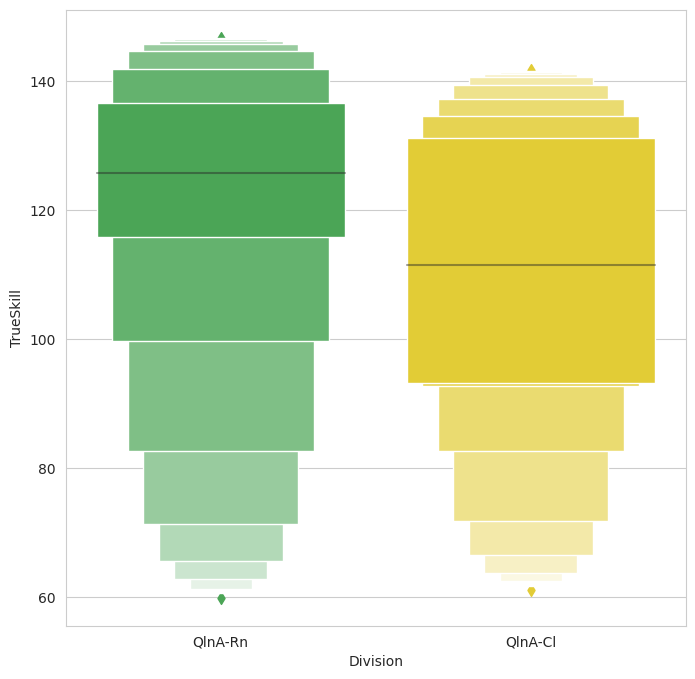
\includegraphics[width=0.45\linewidth]{Results/figures/matchupdistTrueSkill.png}
}
\subcaptionbox{
    Ranked by Mean
}{
    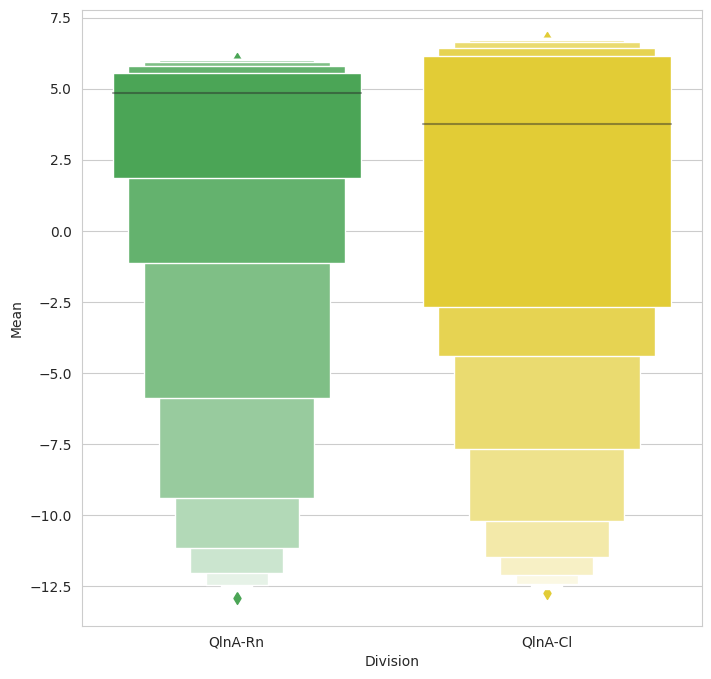
\includegraphics[width=0.45\linewidth]{Results/figures/matchupdistMean.png}
}
\subcaptionbox{
    Ranked by Median
}{
    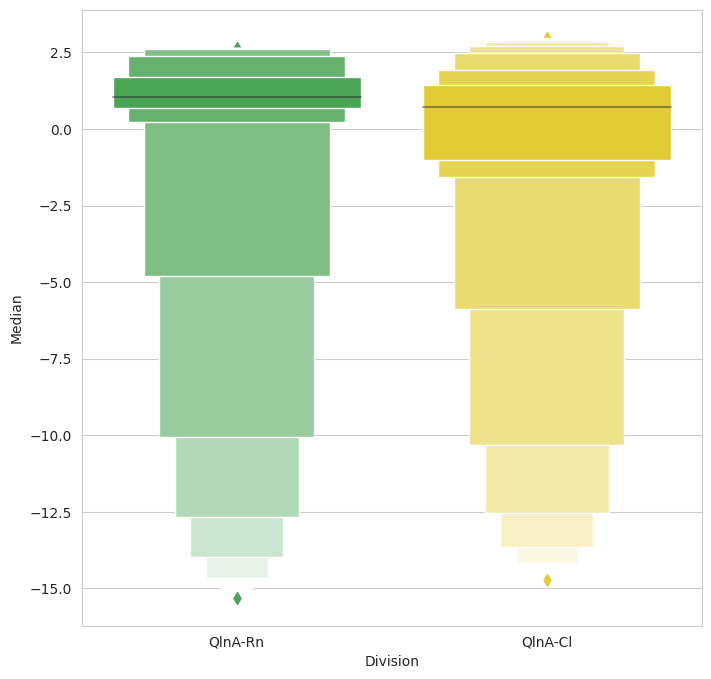
\includegraphics[width=0.45\linewidth]{Results/figures/matchupdistMedian.png}
}
\subcaptionbox{
    Ranked by 20-Percentile
}{
    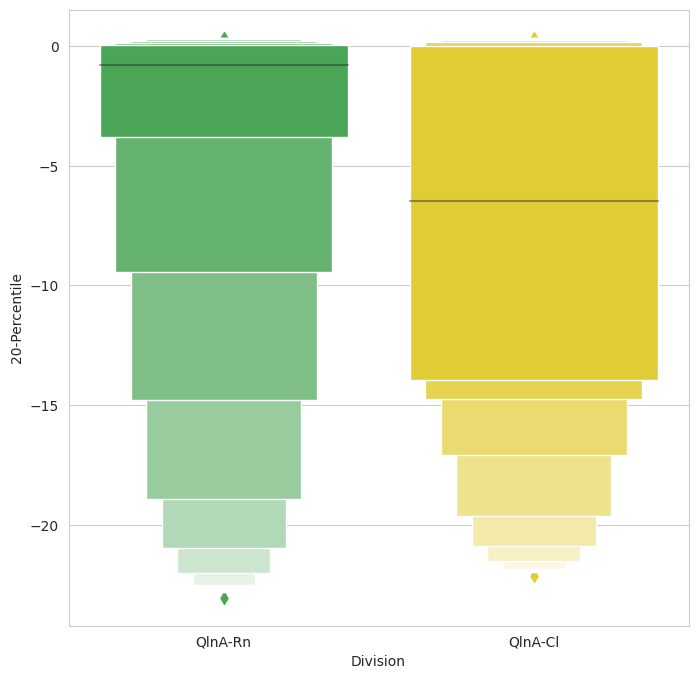
\includegraphics[width=0.45\linewidth]{Results/figures/matchupdist20-Percentile.png}
}
\caption{Agent distribution by matchup type}
\label{MatchupDistribution}
\end{figure}

Figure \ref{MatchupDistribution} takes a closer look at Climbing vs Random for the same agent architecture. Random is more robust in the final evaluation (against all agents), whereas the best Climbing agents earn more money.

\begin{figure}[H]
\centering
\subcaptionbox{
    Qln8-Cl
}{
    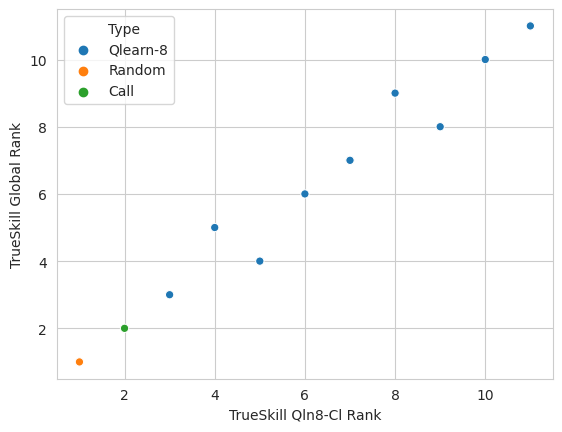
\includegraphics[width=0.45\linewidth]{Results/figures/internal_vs_external_Qln8-Cl.png}
}
\subcaptionbox{
    QlnA-Cl
}{
    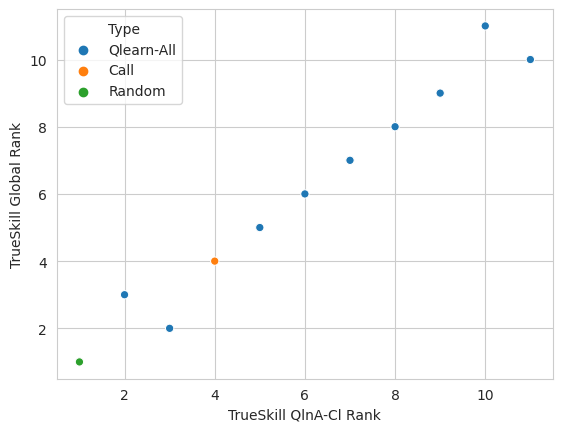
\includegraphics[width=0.45\linewidth]{Results/figures/internal_vs_external_QlnA-Cl.png}
}
\subcaptionbox{
    SacL-Cl
}{
    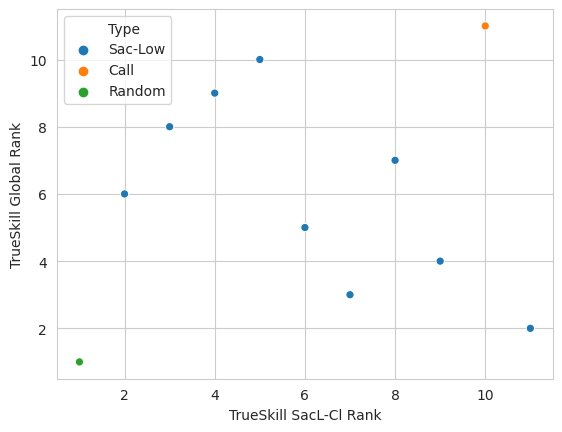
\includegraphics[width=0.45\linewidth]{Results/figures/internal_vs_external_SacL-Cl.png}
}
\subcaptionbox{
    SacH-Cl
}{
    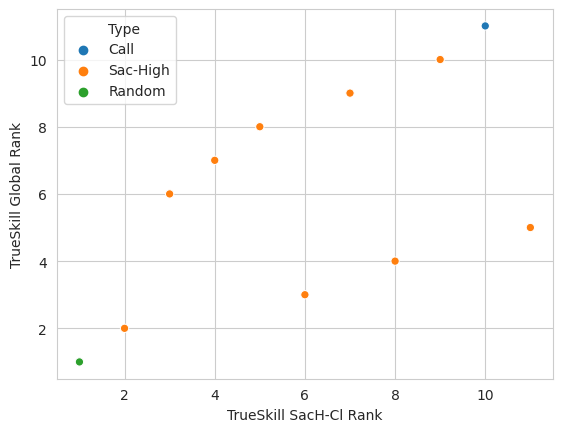
\includegraphics[width=0.45\linewidth]{Results/figures/internal_vs_external_SacH-Cl.png}
}
\subcaptionbox{
    AllAg-Cl
}{
    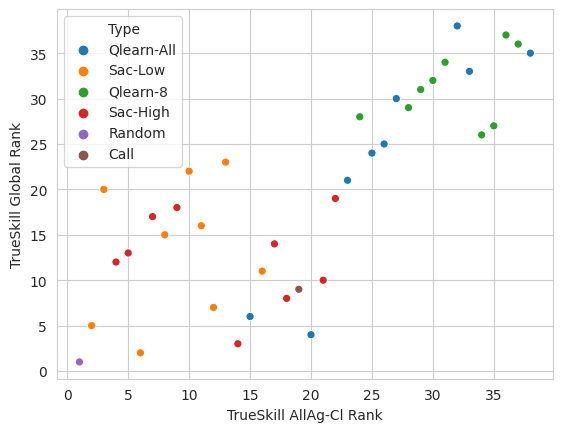
\includegraphics[width=0.45\linewidth]{Results/figures/internal_vs_external_AllAg-Cl.png}
}
\subcaptionbox{
    QlnA-Rn
}{
    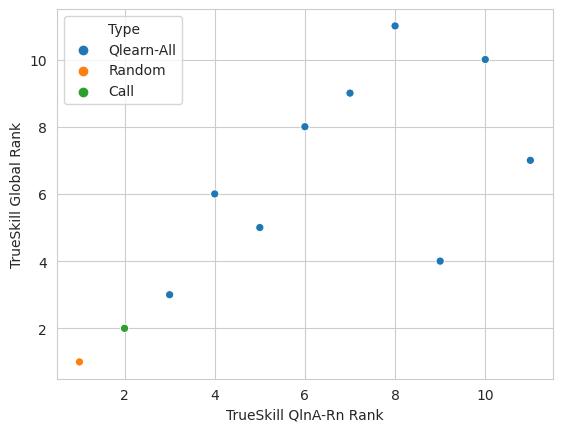
\includegraphics[width=0.45\linewidth]{Results/figures/internal_vs_external_QlnA-Rn.png}
}
\caption{Internal ranking vs PermaEval global ranking by division, colored by agent type}
\label{DivisionConsistency}
\end{figure}

To estimate how much agents in each division overfit, we compared the internal ranking of agents in each division with the global ranking of those agents. Figure \ref{DivisionConsistency} shows this relation. Ideally, the rankings would form a straight line from bottom-left to top-right.

It seems very little overfit happens, as these results echo those of Figure \ref{TrueSkillCompare2}, meaning that most variation here is expected simply due to TrueSkill seed.

One must recall Figure \ref{TrueSkillCompare}, and consider that internal rankings were computed parallel to training. This means the latest agents had only 200 rounds to establish their ranking, and even the oldest less than two thirds of the time compared to the global ranking.